% Created 2021-07-09 Fri 16:06
% Intended LaTeX compiler: pdflatex
\documentclass[11pt]{article}
\usepackage[utf8]{inputenc}
\usepackage[T1]{fontenc}
\usepackage{graphicx}
\usepackage{grffile}
\usepackage{longtable}
\usepackage{wrapfig}
\usepackage{rotating}
\usepackage[normalem]{ulem}
\usepackage{amsmath}
\usepackage{textcomp}
\usepackage{amssymb}
\usepackage{capt-of}
\usepackage{hyperref}
\author{Hsin-Yeh Wu}
\date{\today}
\title{AnaBHEL Single Photon IR detector R\&D}
\hypersetup{
 pdfauthor={Hsin-Yeh Wu},
 pdftitle={AnaBHEL Single Photon IR detector R\&D},
 pdfkeywords={AnaBHEL, black hole, single photon detector, SNSPD, KID, Entanglement, Polarization},
 pdfsubject={Org mode syntax example},
 pdfcreator={Emacs 27.2 (Org mode 9.5)}, 
 pdflang={English}}
\begin{document}

\maketitle
\setcounter{tocdepth}{5}
\tableofcontents


\section*{Overview}
\label{sec:org811364a}

\subsection*{AnaBHEL Description\hfill{}\textsc{Intro}}
\label{sec:orgf61c956}

\begin{figure}[htbp]
\centering
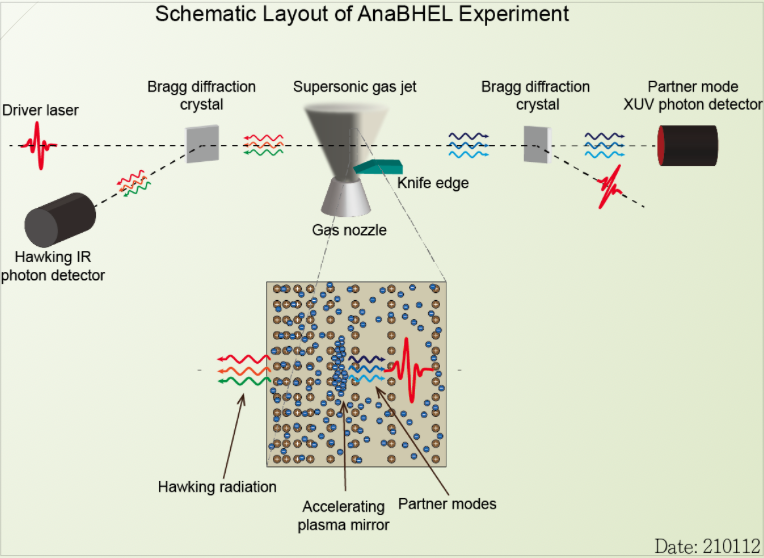
\includegraphics[width=.9\linewidth]{Overview/2021-07-07_19-08-46_2021-07-07_18-49-02_2021-07-07_18-48-24_Screen Shot 2021-07-07 at 6.48.18 PM.png}
\caption{Schematic layout of the AnaBHEL experiment. On the left is where we would receive the expected red shifted Hawking IR photon, and the partner mode would be on the other side which an XUV single photon detector is used. The signal photon pair are extracted from vacuum, therefore entangled and polarization anticorrelated.}
\end{figure}

\subsection*{A review of SPD candidates\hfill{}\textsc{Intro}}
\label{sec:orgf369e68}

\cite{morozov18_super_confer_presen}

\cite{taylor20_mid_confer_presen}

\begin{center}
\begin{tabular}{lllll}
Detector & NEP (W/\sqrt{Hz}) & Single-photon sensitive? & Efficiency & Time Constant\\
\hline
MCT (HgCdTe) & 10\textsuperscript{-19} & Preliminary results & High & \textasciitilde{}100ns\\
SC detectors (KID/TES/HEP) & 10\textsuperscript{-16} & Yes & High & \textasciitilde{}0.01 - 1ms\\
Mid-IR up-conversion & Detector-dependent & Detector-dependent & \textasciitilde{}20\% & Detector-dependent\\
Commercial (InAsSb) & 10\textsuperscript{-11} & No &  & \textasciitilde{}10 μs\\
SNSPD & 10\textsuperscript{-21} & Yes & 20\% (current, 2um) & Free-running, jitter < 90us\\
\end{tabular}
\end{center}

\subsubsection*{SPAD}
\label{sec:orgdfd6d2b}
\subsubsection*{SNSPD}
\label{sec:org627d181}
\subsubsection*{KID}
\label{sec:org065e8d1}

\subsection*{Detector R\&D Flow Chart\hfill{}\textsc{Plan:Intro}}
\label{sec:org8d95ac8}

\begin{center}
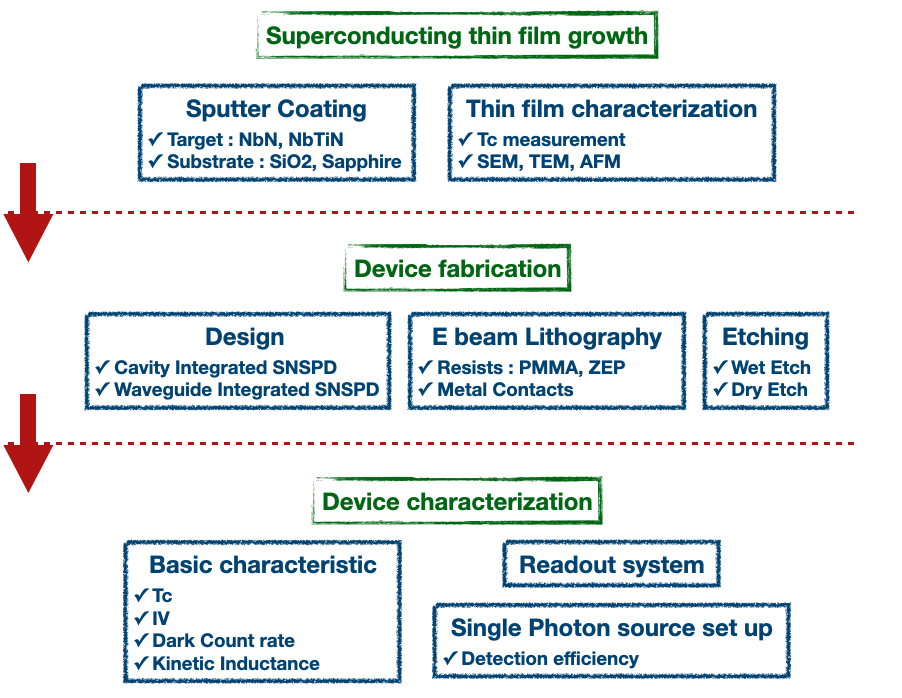
\includegraphics[width=.9\linewidth]{Overview/2021-07-09_15-45-38_Screen Shot 2021-07-09 at 3.45.35 PM.png}
\end{center}

\section*{Todo}
\label{sec:org9bd60d5}
\subsection*{Create shared platform to edit project documents\hfill{}\textsc{General}}
\label{sec:orga81f206}

HI HI

\subsubsection*{{\bfseries\sffamily STRT} Finalize the format}
\label{sec:org7280cca}
\subsubsection*{{\bfseries\sffamily TODO} Create git repository}
\label{sec:org3cd2cdd}

\subsection*{Sputter Coating\hfill{}\textsc{Sputter}}
\label{sec:orgcc03371}

\subsubsection*{First thin film @ NEMS Facility}
\label{sec:orgd1503f1}
Goal: To get familiar with superconducting thin film growing, measure the superconductivity in a cryogenic system. I plan to grow a 300nm Nb film on top of SiO\textsubscript{2} substrate using the sputter machine at NEMS facility.\cite{NEMS_official}

\paragraph*{{\bfseries\sffamily WAIT} Nb \& Ti Target\hfill{}\textsc{Sputter}}
\label{sec:org4b2ca4c}
Ordered with Gredmann group on 2021-06-07

Contact : Bella Leng

Mail : bella.leng@gredmann.com

\href{Todo/2021-07-09\_09-49-32\_Stathes Paganis-1.pdf}{Quotation}

\paragraph*{{\bfseries\sffamily TODO} Substrate\hfill{}\textsc{Sputter}}
\label{sec:org7dc2137}

\paragraph*{{\bfseries\sffamily TODO} Discuss Parameters}
\label{sec:org48bf91e}

\section*{Device Fabrication}
\label{sec:orgc35bfb3}
Here are the needed fabrication and experiment steps for building SNSPD. Many parts is inspired of the work from Glasgow University group, and modified to the equipment we have here.
\cite{erotokritou19_next_gener_super_nanow_singl_photon_detec}

\subsection*{Sputter}
\label{sec:org684b5a1}
\subsection*{E beam Lithography}
\label{sec:orgb9bc14a}

\subsection*{Etching}
\label{sec:org85486c8}

\section*{Experimental Methods}
\label{sec:orgb2f1dd4}
\subsection*{Cryogenic system\hfill{}\textsc{Cryogenic}}
\label{sec:org3df5165}
\subsection*{Tc measurement\hfill{}\textsc{Cryogenic:Characteristic}}
\label{sec:org0338002}
\subsection*{SEM\hfill{}\textsc{Characteristic}}
\label{sec:org7eddc9e}
\subsection*{Readout system\hfill{}\textsc{DAQ}}
\label{sec:org2d89c5c}
\subsection*{Single Photon source\hfill{}\textsc{Characteristic:SinglePhoton}}
\label{sec:org8176900}
\section*{Log}
\label{sec:orgd4cd48f}
\subsection*{2021-07-07 Sputter cost discussion\hfill{}\textsc{Sputter}}
\label{sec:org6c6ed9a}
We have two options:
\begin{enumerate}
\item Get 50\% discount everytime we use.
\item Get us a period of free operation time
\end{enumerate}

Estimate cost for one thin film : 1k NTD

\section*{Reference}
\label{sec:orge875147}

\bibliographystyle{unsrt}
\bibliography{../../references/reference}
\end{document}
